\chapter{Knowledge-Based System Integration in a Deep Learning Environment}
\label{chap:kbsintegrationdl}
\textit{The content of this chapter is based on the work \cite{amadoretalontodl}}
\section{Introduction}
\elvitodo{Aquí pos la motivación un poco, limitaciones concretas de esto y por qué}
%Motivaciones de esto: Incrementar capacidad de generalización, reducir número de recursos, aumento de la interpretabilidad del modelo. Restricciones de esto: 


\begin{figure}[ht]
    \centering
    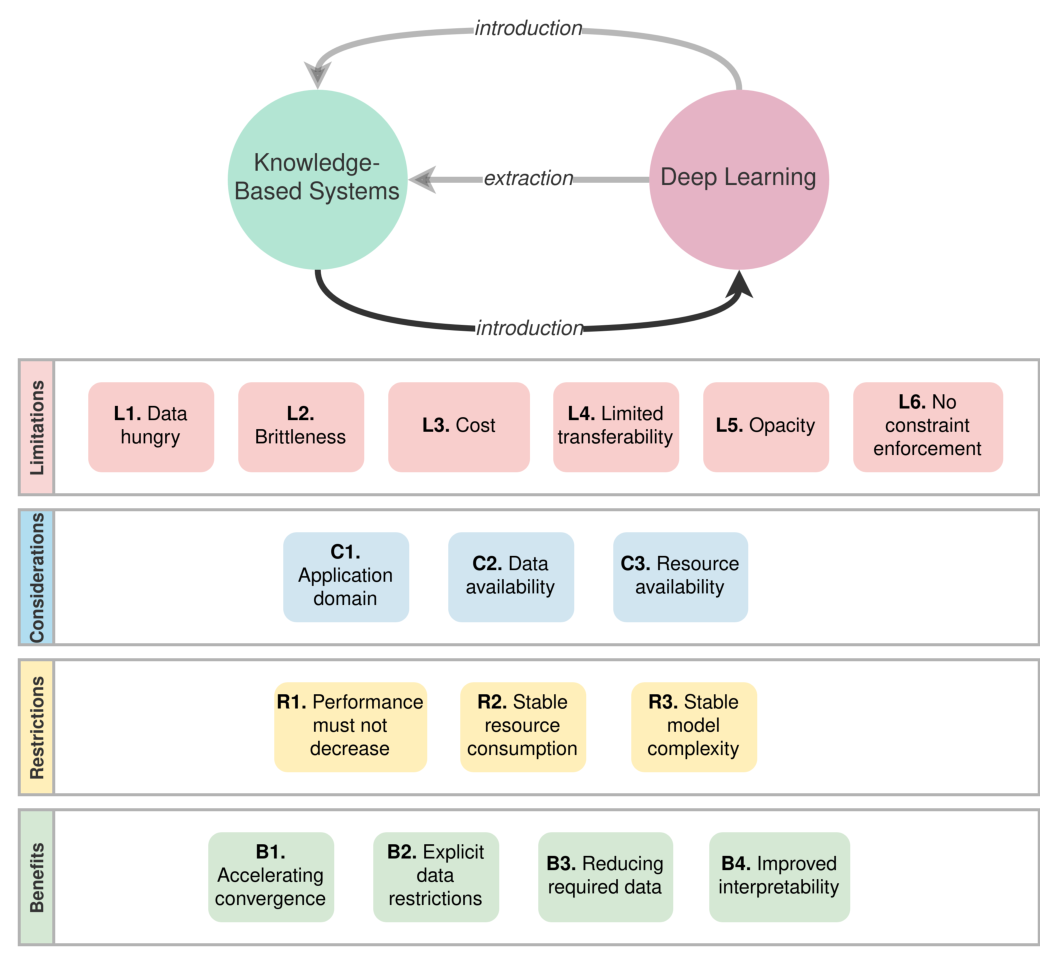
\includegraphics[width=\linewidth]{4_kbsintegrationdl/figures/overview_kbs_dl_intro.eps}
    \caption{Overview on the Introduction of Knowledge-Based Systems into Deep Learning}
    \label{fig:overview_kbs_dl_intro}
\end{figure}

%%%LA MOVIDA DE LA SENSIA EN ESTA VERTIENTE CONCRETA
\section{Knowledge-Based System Introduction in Deep Learning Models} \label{subsec:methods_dl}
In this scenario, the DL model plays the primary role, while the KBS plays the secondary role. Figure \ref{fig:overview_kbs_dl_intro} outlines the specific methodological parameters for this integration, which are defined as follows.
\elvitodo{AMPLIAR}

\subsection{Limitations}
\begin{enumerate} [start=1,label={\bfseries L\arabic*.}]
    \item \label{kbsintrodl_L_data_hungry} \textbf{Data hungry.} This is one of the most concerning issues regarding DL. While DL models are capable of achieving an abstraction and generalization capacity that can not be modelled by their symbolic counterpart, their final performance is highly linked to both the quality and the quantity of the data. Large, balanced and representative training sets are required for the DL model to learn valid reasoning patterns about the data. This limitation implies that the final performance of the model is directly bounded to its training data, thus not being a trusty indicator on the aptness of the model. 
    
    \item \label{kbsintrodl_L_brittleness} \textbf{Brittleness.} DL models infer abstract reasoning patterns from input training data. These patterns, however, may not be robust enough to correctly deal with noisy input data. Adversarial attacks can cause DL models to fail. Therefore, even if a given DL produces an output $Y$ for a given input $X$, it can not be ensured that for a slightly corrupted version of the input $X'$ will lead to the same outcome.
    
    \item \label{kbsintrodl_L_cost} \textbf{Cost.} Training a DL model requires an elevated computational cost. While GPUs have greatly alleviated this issue, the disparity on the availability of computational resources is a significant drawback of DL models. Not only the training time varies greatly across different infrastructures for the same implementation, but a given DL model may be incapable of training or executing if the available resources are insufficient. Maintaining computational cost at reasonable limits should therefore be prioritized.  
    
    \item \label{kbsintrodl_L_transfer} \textbf{Limited transferability.} Reusability is one of the most prominent features of DL models. Transfer learning reduces the need to retrain a given architecture from scratch to fit a new dataset or solve a new task. However, a model $M$ may achieve a remarkable performance on a given task $t$, but this performance may not  hold for a different task $t'$, even if they are fairly similar. Additionally, if a model $M'$ is trained using $M$ as a base, it can not be ascertain whether the performance of the newly trained model will be as good as the baseline one.
    
    \item \label{kbsintrodl_L_opacity} \textbf{Opacity.} As outlined in Section \ref{sec:sota_knowledge_extraction_dl}, one of the main concerns regarding DL models is their limited explainability. DL models are often provide better results than KBS on multiple tasks, but their usage is often hindered due to the impossibility to provide human-understandable insights on why a certain output is obtained.
    
    \item \label{kbsintrodl_L_constraint} \textbf{No constraint enforcement.} DL models infer patterns from a set of input samples. However, these patterns may not truthfully represent the data, as noisy or unbalanced data may negatively impact the learning process. The patterns learned by a DL model can then be inconsistent, and may not be able to properly generalize for unseen inputs.
    \end{enumerate}
\subsection{Considerations}
\begin{enumerate} [start=1,label={\bfseries C\arabic*.}]
    \item \label{kbsintrodl_C_domain} \textbf{Application domain.} The conducted systematic review \citep{amador_systematic_review_2019} showcased an existing bias in the employed reasoning models per application domain. Complex and opaque approaches were selected in domains where their worst-case scenario impact was low (i.e. housing), while fully expressive and interpretable models were considerably favoured in human-dominated areas (i.e, healthcare). Therefore, in this scenario where the DL model is the primary, it must be studied whether the application domain strictly requires from human understandability. Even though the introduction of KBS into DL models may reduce its opacity, it may not be sufficient to fully comprehend the inference process of the model. 
    
    \item  \label{kbsintrodl_C_data} \textbf{Data availability.} As stated in \ref{kbsintrodl_L_data_hungry}, data availability is one of the main bottlenecks of DL models. This issue may be alleviated by the introduction of a KBS model. In those scenarios where the KBS model is already trained, data availability may not be an issue. However, if the KBS model needs to be trained before being integrated within the DL model, there must exists valid data to build the KBS model. Data availability for KBS model training must then be ensured beforehand.
    
    \item  \label{kbsintrodl_C_resource} \textbf{Resource availability.} This consideration is directly related to \ref{kbsintrodl_L_cost}. KBS models have a much reduced computational cost in comparison to DL models. However, even if small, they still carry a computational cost that is added to the baseline cost of the DL model which should be noted. The cost of introducing the KBS model should never exceed the cost of the primary DL model.
    
\end{enumerate}
\subsection{Restrictions}
\begin{enumerate} [start=1,label={\bfseries R\arabic*.}]
    \item \textbf{Performance must not decrease.} One of the fundamental strengths of DL models is that they provide remarkable performances on a wide variety of tasks. The introduction of a KBS model must never negatively impact the performance of the model, as this is a pivotal element and should therefore be preserved. While there may not be a remarkable improvement in the final metrics (i.e., a set of rules to correctly predict outliers, which may represent a very small fraction of the data), the performance should, at least, remain stable.
    
    \item \textbf{Stable resource consumption.} The introduction of an additional model subsequently carries an additional cost. As noted in \ref{kbsintrodl_C_resource}, this increment must be taken into consideration. The overall resource consumption of the model must remain within reasonable bounds (\ref{kbsintrodl_L_cost}). 
    
    \item \textbf{Stable model complexity.} 
\end{enumerate}
\subsection{Benefits}
\begin{enumerate} [start=1,label={\bfseries B\arabic*.}]
    \item \textbf{Accelerate convergence}
    \item \textbf{Explicit data restrictions.}
    \item \textbf{Reduce required data.}
    \item \textbf{Improved interpretability.}
\end{enumerate}
%Limitaciones y las restricciones estudiadas
%Limitaciones: necesidad de reentrenamiento para incluir un único elemento, data hungry, tendencia a la personalizacion, necesidad de grandes recursos computacionales + los que se identifiquen en bibliografía
\elvitodo{Aquí hay mucha magra en el paper de Frank y las referencias de ese paper}

\section{Ontology Introduction on Knowledge Graph Embedding Models for Knowledge Graph Completion} \label{subsec:ontointro_kgc}

This Section provides a case scenario of an introductory integration of symbolic knowledge under a deep learning framework, as presented in \cite{amadoretalontodl}. This case scenario focuses on the Knowledge Graph Completion (KGC) task, specifically on its resolution via Knowledge Graph Embedding (KGE) models. As stated in Section \ref{sec:the_ai_spectrum}, KGE models generate vector representations for KGs, subsequently enabling statistical reasoning over the KG. Figure \ref{fig:box_krintodl_base} depicts the baseline design of any KGE model according to the design patterns in \cite{boxologyfrank}. In this scenario, a KG (structured, symbolic) serves as input. As previously described, a KG is represented as a set of facts of the format \textit{(s,p,o)}, where $s,o \in \mathcal{E}$ and $r \in \mathcal{R}$. Following the standard model generation procedure, the input is divided into three separate subsets of facts: training, validation and test, each containing a different set of facts from the KG. The training set is then fed into a KGE model, which generates a subsymbolic representation for each element of the input. These vector representations can then be used to infer new potential elements of the KG. 

\begin{figure*}
    \centering
    \includegraphics[width=\linewidth]{4_kbsintegrationdl/figures/boxology_krintodl_base.png}
    \caption{Boxology representation of the baseline KGE model}
    \label{fig:box_krintodl_base}
\end{figure*}


While this method provides an efficient solution to the KGC task, two main shortcomings can be identified: (1) they only rely on the information explicitly declared in the input data, thus not considering background, general information that can lead to the inference of general restrictions about the output and (2) they cannot reason over inputs that were not seen by the model during training time.\elvitodo{RELACIONAR ESTO CON LAS LIMITACIONES GENERALES QUE TENEMOS QUE DECLARAR}. One of the main reasons behind these flaws is the training strategy employed by KGE models, as they rely on a local search strategy instead of a explorative one. Therefore, scalable and explorative approaches are needed to reason over the so-called \textit{out-of-knowledge-based} (OOKB) entities. This term is employed to refer to entities that were not featured in the training set and, therefore, have no learnt representation. 

A feasible solution to this issue lies in the inclusion of explicit ontological information, as explored in \cite{Patrick}. As ontologies are a core element of the KG, serving as a scaffold for its generation as well as providing explicit restrictions about entities and relations. However, their use scope is limited exclusively to the generation and introduction of new elements of the KG \citep{paulheim2017knowledge}. Existing proposals regarding OOKB entity introduction include works such as \textit{puTransE} by \cite{putranse}, \textit{DKGE} by \cite{dkge}, \cite{hamaguchi_etal} and \cite{shah_open-world_2019}. These proposals, however, rely on deep learning models, thus suffering from some of the limitations outlined in Section \ref{subsec:limitations_dl}, namely \elvitodo{REFERENCIAR LIMITACIONES EXACTAS DE LA LISTA ANTERIOR}. This chapter presents a simpler, hybrid alternative to the aforementioned works, which eliminates the detected limitations while being easily integrated with any existing KGE model.

KGE models assign a singular representation for each entity and relation which encode all the knowledge about the input derived from the training facts. While every entity is unique and this must be reflected into its representation, certain generalizations about them can be stated from the existing facts. Ontologies encode these generalizations and restrictions, and its inclusion alongside KGE models can enable the extraction of general patterns about the facts while still maintaining the specificity of the entities and relations. Additionally, ontologies play a key role on entity introduction, thus making this information about new entities easily available.

\begin{figure}
    \centering
    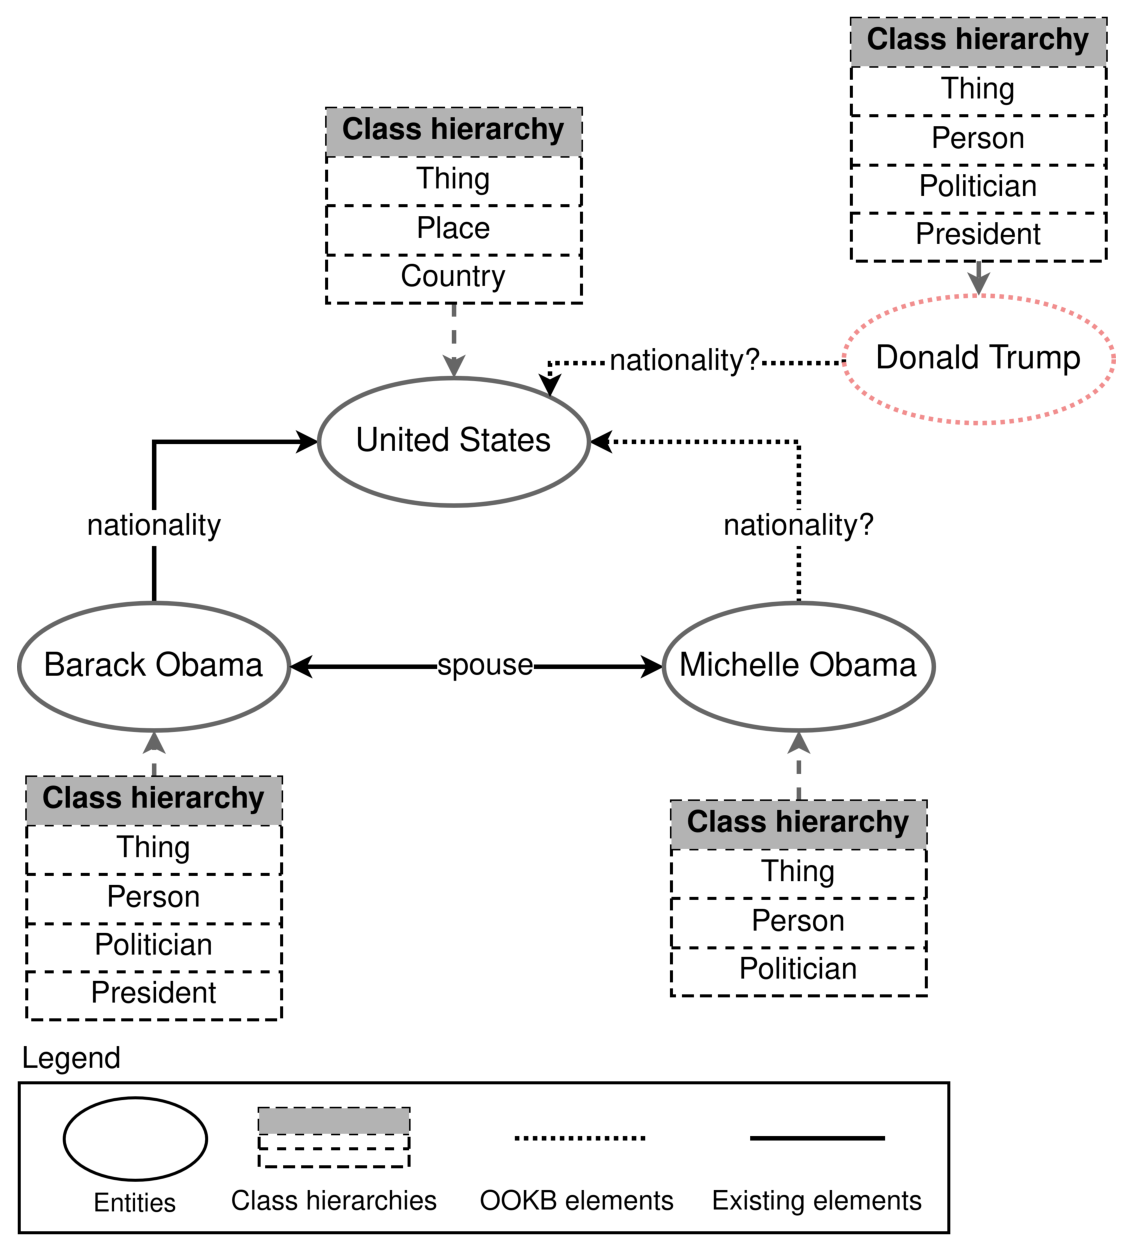
\includegraphics[width=.8\linewidth]{4_kbsintegrationdl/figures/KGCexample.eps}
    \caption{An example of KGC combining entity information and hierarchical information. Boxes limited by dashed lines represent the ontological information of the entity. Dotted lines are used to represent unknown information.}
    \label{fig:kgc_onto_example}
\end{figure}

Figure \ref{fig:kgc_onto_example} outlines the general idea of the proposal. Every entity contains its own ontological information. In this example, the class hierarchy of each entity is used as ontological information. While facts about a given entity $e$ are volatile and subject to change, its class hierarchy remains fairly static throughout time. Moreover, class hierarchies are similar or even equal in those entities representing closely related concepts. In the depicted entities "Barack Obama" ($e_1$) and "Donald Trump" ($e_2$), their class hierarchies are equal, implying that they represent the same type of concept. For the entity "Michelle Obama", its class hierarchy is a subset of the class hierarchy of the aforementioned entities. Therefore, even though this entity does not represent a "President", it still holds a high resemblance with both $e_1$ and $e_2$. Considering the equality of the class hierarchies of entities $e_1$ and $e_2$, even though $e_2$ was not featured in the training set, analogical inference can be performed. The combination of the ontological background of the entity with its specific information makes it possible to leverage information about similar entities, leading the model to infer non-explicit restrictions capable of enable reasoning over OOKB entities. In the example depicted in Figure \ref{fig:kgc_onto_example}, even though the only known information about the entity "Donald Trump" is its class hierarchy, it can be assessed whether the potential fact \textit{(DonaldTrump, nationality, UnitedStates)} holds based on its resemblance with the known fact \textit{(BarackObama, nationality, UnitedStates)}. 




\section{Semantic-Based Initialization for Out-Of-Knowledge-Base Entity Reasoning}
\begin{figure*}
    \centering
    \includegraphics[width=\linewidth]{4_kbsintegrationdl/figures/boxology_krintodl.png}
    \caption{Boxology representation of the proposed hybrid KGE model. Dotted lines depict added elements. A red square outlines the initialization.}
    \label{fig:box_krintodl}
\end{figure*} 

Even though the introduction of ontological information solves the issue of OOKB entity reasoning, specific information about the unseen entities is also required to properly typify them. Moreover, unseen entities need to be represented in the same format as known entities in order to be processed by the KGE model. Figure \ref{fig:box_krintodl} shows the boxology representation of the proposed approach. Instead of directly feeding a set of facts in relational format to the KGE model like in the baseline model, an additional transformation layer is added to perform initialization (depicted as a red box). The proposed initialization method encodes not only ontological information, but semantic, specific knowledge about each of the entities. From a formal representation standpoint, the proposed hybrid model may be perceived as more complex due to its increased number of boxes. However, it is worth noticing that the initialization is performed offline, thus not adding any complexity to the KGE model itself \elvitodo{Referenciar con las assumptions que tenemos al respecto?}. Figure \ref{fig:overview} depicts the three phases of the initialization: \textbf{ontology retrieval}, \textbf{background knowledge encoding} and \textbf{embedding composition}.

 
% The incremental six-step initialization procedure is depicted in Figure \ref{fig:overview}. These steps can be grouped into three different phases: \textbf{entity information retrieval, embedding generation} and \textbf{performance evaluation}

\begin{figure}
    \centering
    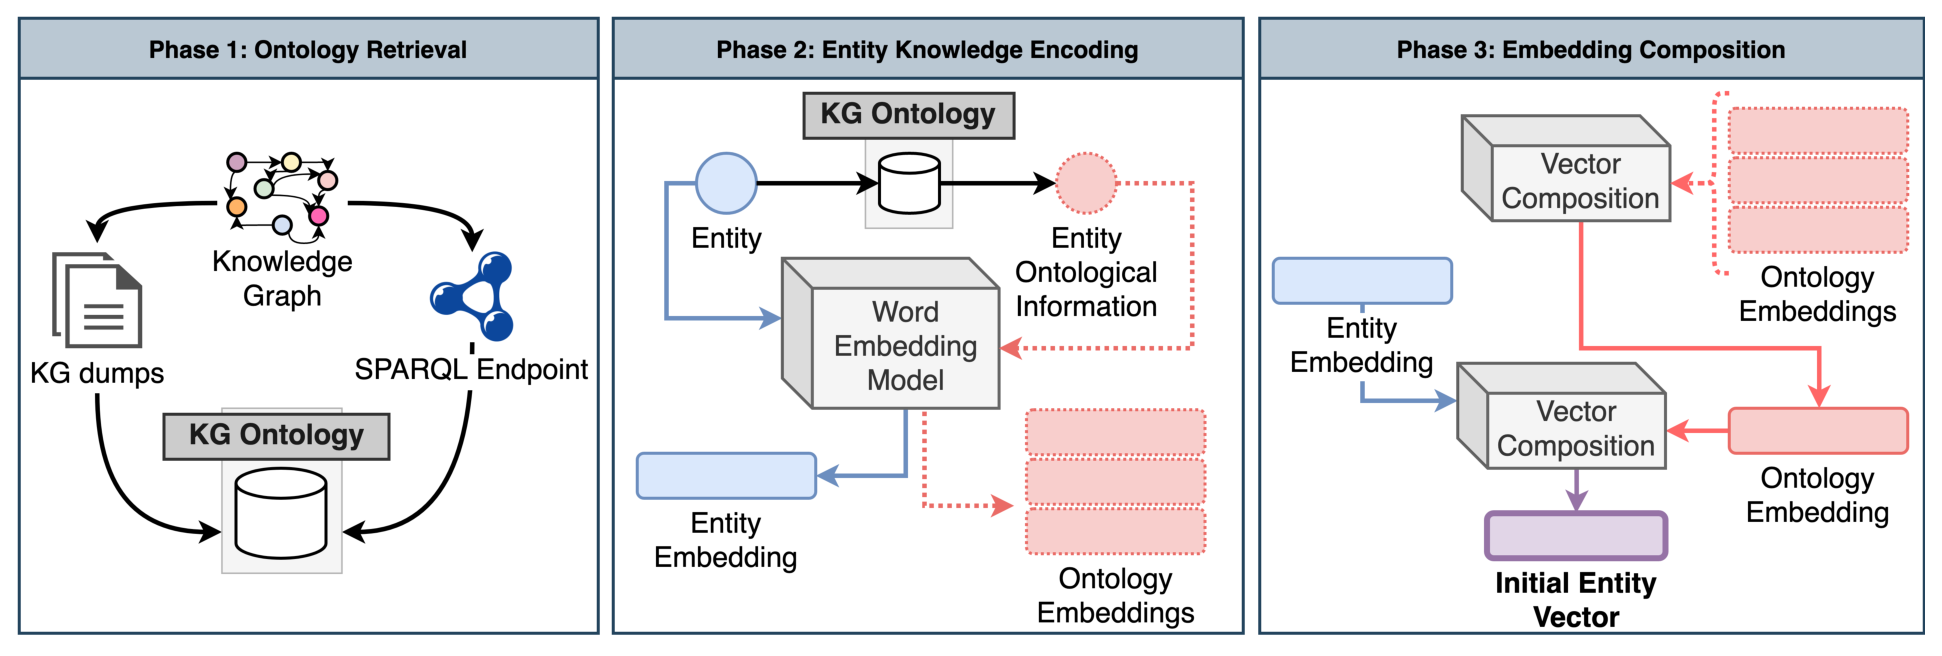
\includegraphics[width=\linewidth]{4_kbsintegrationdl/figures/Initialization_phases.eps}
    \caption{Overview of the three initialization phases}
    \label{fig:overview}
\end{figure}

% Figure \ref{fig:overview} showcases the proposed incremental six-step procedure conducted to initialize and reason over OOKB entities. 
% \elvitodo{A lo mejor esa figura se podría modernizar, que está fea} These steps can be categorized into three phases: entity information retrieval, embedding generation and performance evaluation.

\subsection{Ontology Retrieval}
Opposite to the volatility of KGs, ontologies provide stable, general information. Their role in the generation of KGs is crucial but their application scope is usually limited to the introduction and creation of new elements of the graph. The information encoded in ontologies can be particularly beneficial cor KGC, as they provide explicit restrictions about the type of entities featured on each relation, as well as additional information that can enhance the inference process of the models.

Ontologies comprise the following parts: individuals, classes, properties, relations, function terms, restrictions, rules, axioms and events. Only individuals (or entities in the context of KGs), relations and properties are considered by KGE models on the generation of representations. Therefore, a substantial amount of components that could greatly enhanced the final quality of the embeddings is dismissed.

Class hierarchies are at the core of both ontologies and KGs. During the introduction, entities are grouped into the class that better represents them conceptually. These classes are not atomic, but form a tree-like hierarchical structure, ranging from the most specific (or \textit{leaf}) classes to the \textit{root} class, which is shared by all entities in the graph. This taxonomical structure enables fine-grained distinctions between conceptually similar classes, as in Figure \ref{fig:kgc_onto_example}, where the entities "Barack Obama" and "Michelle Obama" are both \textit{Politicials}, but the first one is also a \textit{President}. Therefore, it provides a trade-off between the generality of the tree-like structure with the specificity of the different subclasses. 

While classes provide a general and unified framework, properties provide distinct, unique information about entities. KG facts are usually extracted from the interaction between two individuals by means of a property. Properties that relate an individual with a non-individual (i.e: a numerical value, a description, etc.) are usually discarded, even though this information could further enrich the final embeddings. Rules and axioms can also be encoded within the KGE model. In this case, axioms can be used to guide the training of the KGE model, ensuring that the predictions made from the model are consistent. Additionally, rules can also be used for training data augmentation, as new facts may be inferred from the existing KG. The newly inferred facts can then also be included as part of the training set.

Restrictions are also closely related with KGE, as relation representations encode implicit constraints about the expected types of head and tail entities. However, the restrictions inferred by KGE models have a local scope, as they are based only on the facts contained in the training set. Therefore, these constraints may not be applicable to every fact that features the relation. Explicit restrictions about the relations can also be encoded jointly with their representations to deal with this shortcoming, improving the performance of the model on KGC.

Phase 1 of Figure \ref{fig:overview} showcases the two different available paths for ontology retrieval: KG dumps or SPARQL queries. Currently, most of the publicly available KGs provide their data dumps, which includes not only the KG facts, but its ontology file as well as extra documentation. Furthermore, every entity and relation encoded in the KG is explicitly related to its corresponding ontological information, reducing the retrieval time. However, data dumps usually come compressed in a single file that can scale up to several terabytes, which can be undesirable in terms of computational resources. KGs usually provide a SPARQL endpoint, which enables information retrieval via queries. This approach is more efficient, as fewer resources are required and the target information can be retrieved directly with a single query. Nonetheless, using SPARQL queries may be discouraged in cases where the KG has a large size or if the number of SPARQL queries is elevated. 

\subsection{Background Knowledge Encoding}
The first phase of the proposed initialization focuses on obtaining all the background knowledge (both ontological and specific) required to fully typify an entity. While the existing OOKB entity reasoning approaches presented in Section \ref{subsec:ontointro_kgc} are capable of generating highly representative embeddings, these representations lack any semantic information about the entity itself. Semantic information is highly relevant in this context, as it enriches the entity embeddings with an additional level of knowledge that can not be inferred otherwise from the input. Despite this fact, most KGE models still rely on random initialization. 

One-hot vectors are an easy and straightforward replacement to random initialization. In this encoding, each entity is embedded as a vector of dimension $N$, where $N$ is the total number of entities. For every entity, a single vector can be created composed entirely of zeros expect for a single one value in a given position, which is unique to each entity. While this encoding may be suitable for small KGs, it cannot be applied to large inputs, as the simension of the embedding grows linearly with the size of the KG. Moreover, zero-valued initializations can hinder the convergence of the model to its optimal solution, and they do not encode semantic information about the entity.

Word embeddings provide a preferable initialization alternative. These methods are capable of generating expressive, unique representations for the words in a vocabulary. Different paradigms can be identified amongst word embedding models for the representation of words. Word2Vec \citep{word2vec} generates a single representation per token in the vocabulary, which hinders the representation of unseen words. FastText \citep{fasttext1,fasttext2} considers each word as a set of subparts called n-grams, assigning a representation for each of them. The final representation of a word is composed by the average of this n-grams. While FastText is capable of representing words that were not in the training corpus and still enable analogical reasoning, it still lacks the capability of correctly model polysemy. Language models, such as ElmO \citep{elmo} or BERT \citep{bert} solve all of the aforementioned issues, but the dimension of the resulting embeddings increases noticeably. Word2Vec embeddings tend to have a length of about 300, which scales up to 2048 on BERT. This dimension conflicts the regular dimension of KGE vectors, which rarely exceed 200. Dimensionality reduction based on \textit{principal component analysis} \citep{dim_reduction} is a potential solution to the mismatch between the dimensions of KGE and word embedding outputs. However, it is noticeable that reducing the dimension of word embedding directly affects its final expressivity. 

Another importan dissimilarity between word and KG embeddings is that whereas word embeddings follow a token-based approach, KGE models are oblivious to the number of tokens that name an entity. Therefore, a composition method is needed that guarantees that all the tokens that compose an entity are represented on its initial embedding. Following the same criteria employed in FastText to compose the final representation of a word, averaging the single representations of each token 


% \elvitodo{Empezar a hablar de inicializacion de Word Embeddings}

\subsection{Embedding Composition}


\section{Experimentation}
\section{Discussion}





\section{Summary}